%%%%%%%%%%%%%%%%%%%%%%%%%%%%%%%%%%%%%%%%%
% Classicthesis-Styled CV
% LaTeX Template
% Version 1.0 (22/2/13)
%
% This template has been downloaded from:
% http://www.LaTeXTemplates.com
%
% Original author:
% Alessandro Plasmati
%
% License:
% CC BY-NC-SA 3.0 (http://creativecommons.org/licenses/by-nc-sa/3.0/)
%
%%%%%%%%%%%%%%%%%%%%%%%%%%%%%%%%%%%%%%%%%

%----------------------------------------------------------------------------------------
%	PACKAGES AND OTHER DOCUMENT CONFIGURATIONS
%----------------------------------------------------------------------------------------

\documentclass{scrartcl}

% \usepackage[top=2in, bottom=1.5in, left=0in, right=0in]{geometry}

\reversemarginpar % Move the margin to the left of the page 

\newcommand{\MarginText}[1]{\marginpar{\raggedleft\itshape\small\color{Mahogany}#1}} % New command defining the margin text style

\usepackage[nochapters]{classicthesis} % Use the classicthesis style for the style of the document
\usepackage[LabelsAligned]{currvita} % Use the currvita style for the layout of the document

\usepackage[T1]{fontenc}
\usepackage{graphicx}
\usepackage{ragged2e}

\renewcommand{\cvheadingfont}{\LARGE\color{Mahogany}} % Font color of your name at the top

\usepackage{hyperref} % Required for adding links	and customizing them
\hypersetup{colorlinks, breaklinks, urlcolor=Mahogany, linkcolor=Mahogany} % Set link colors

\newlength{\dateboxperso}\settowidth{\dateboxperso}{Spring 2011} % Set the width of the date box in each block
\newlength{\datebox}\settowidth{\datebox}{Spring 20112222222} % Set the width of the date box in each block

%CHANGE MARGIN
\newenvironment{changemargin}[2]{%
  \begin{list}{}{%
    \setlength{\leftmargin}{#1}%
    \setlength{\rightmargin}{#2}%
  }%
  \item[]}{\end{list}} 

\newcommand{\NewEntryPerso}[3]{\noindent\hangindent=2em\hangafter=2 \parbox{\dateboxperso}{\small \textit{#1}}\hspace{1.5em} #2 #3 % Define a command for each new block - change spacing and font sizes here: #1 is the left margin, #2 is the italic date field and #3 is the position/employer/location field
\vspace{0.5em}} % Add some white space after each new entry

\newcommand{\NewEntry}[3]{\noindent\hangindent=4em\hangafter=0 \parbox{\datebox}{\small \textbf{\textit{#1}}}\hspace{1.5em} #2 #3 % Define a command for each new block - change spacing and font sizes here: #1 is the left margin, #2 is the italic date field and #3 is the position/employer/location field
\vspace{0.3em}} % Add some white space after each new entry

\newcommand{\Description}[1]{\hangindent=4em\hangafter=0\noindent\raggedright\small{#1}\par\normalsize\vspace{1em}} % Define a command for descriptions of each entry - change spacing and font sizes here

%----------------------------------------------------------------------------------------
\usepackage[verbose]{geometry}
\geometry{innermargin=130pt,top=48pt,
  textwidth=400pt,textheight=750pt,
  marginparwidth=1.5in,marginparsep=-0.3in,
  heightrounded}

\begin{document}
\date{}
% \areaset[0.75in]{5.7in}{10.5in}
% \setlength{\marginparwidth}{1.6in}
% \setlength{\marginparsep}{-0.3in}
%----------------------------------------------------------------------------------------
%	NAME AND CONTACT INFORMATION SECTION
%-------------------------------------------------------------------------------
\thispagestyle{empty} % Stop the page count at the bottom of the first page
\begin{cv}{%\spacedallcaps{\textnormal{Bhargav} P. Swaminathan}\\
\textls[140]{Bhargav\ \ Prasanna\ \ SWAMINATHAN}\\
{\large PhD Student\ \ $\cdotp$\ \ Teaching Assistant\ \ $\cdotp$\ \ University of Grenoble-Alps}}\vspace{1.5em} % Your name

\MarginText{\centering 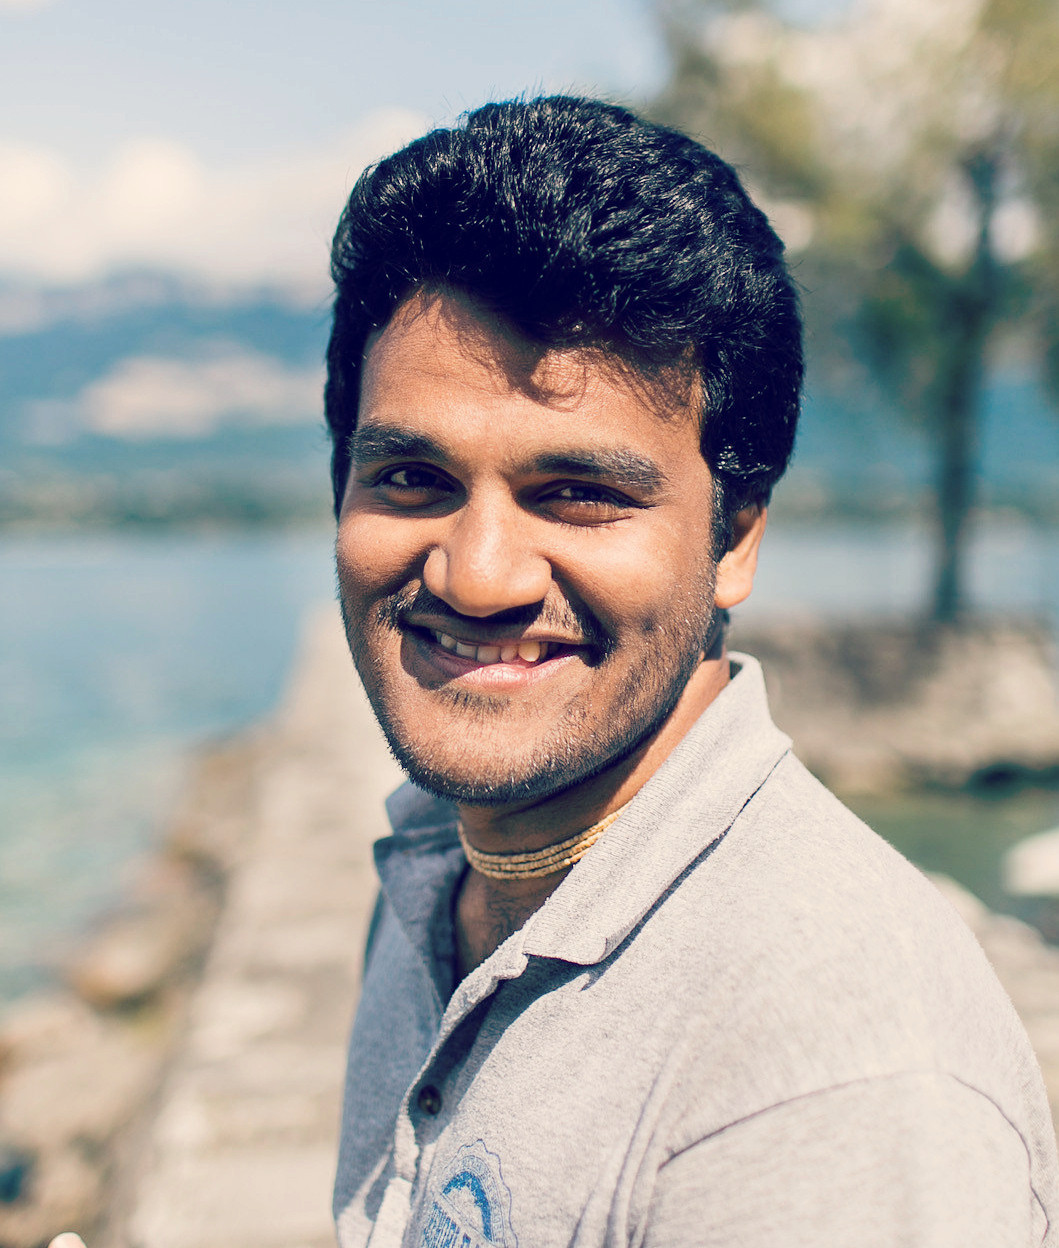
\includegraphics[height=3.2cm]{photo3} \hfill}

\setlength{\marginparsep}{-0.15in}
\vspace{-0.7em}
\noindent\spacedlowsmallcaps{Personal Information}\vspace{0.5em} % Personal information heading

\NewEntryPerso{}{\textit{Born in Chennai, India,}}{17 September 1990} % Birthplace and date

\NewEntryPerso{email (work)}{\href{mailto:bhargav-prasanna.swaminathan@g2elab.grenoble-inp.fr}{bhargav-prasanna.swaminathan@g2elab.grenoble-inp.fr}}

\NewEntryPerso{address}{49 Avenue Alsace Lorraine, 38000 Grenoble, France} % Personal website

\NewEntryPerso{phone}{(H) +33 (0)4 76 17 22 70\ \ $\cdotp$\ \ (M) +33 (0)6 45 85 48 97} % Phone number(s)

\NewEntryPerso{website}{\href{http://bswam.in}{http://bswam.in}}

\NewEntryPerso{linkedin}{\href{http://fr.linkedin.com/in/bhargavswaminathan}{http://fr.linkedin.com/in/bhargavswaminathan}}

\NewEntryPerso{github}{\href{http://www.github.com/rpmdebslack}{http://www.github.com/rpmdebslack}}

\vspace{1em} % Extra white space between the personal information section and goal

\noindent\spacedlowsmallcaps{Career Goal}\vspace{1em} % Goal heading, could be used for a quotation or short profile instead

\Description{To be at the forefront of research in the area of electrical distribution network optimization and integration of distributed generation.}\vspace{0.75em} % Goal text

%----------------------------------------------------------------------------------------
%	WORK EXPERIENCE
%----------------------------------------------------------------------------------------

\noindent\spacedlowsmallcaps{Work Experience}\vspace{1em}

\NewEntry{Feb-Apr 2015}{Visiting Researcher\MarginText{VITO - The Flemish Inst. for Technological Research, Mol, Belgium}}

\Description{Developed economic models for short-term use of flexibility levers in \textsc{mv} electrical distribution networks in collaboration with researchers in the Energy Technology department of VITO. Developed a merit-order routine for evaluating the best use of these flexibilities. The collaboration was as part of the evolv\textsc{dso} project.\\
% \ \\
% \begin{tabular}{rl}
% Reference: & Jean-Yves \textsc{Voyant}\ \ $\cdotp$\ \ +33 (0)4 76 82 63 49\\
% &\href{mailto:jean-yves.voyant@g2elab.grenoble-inp.fr}{jean-yves.voyant@g2elab.grenoble-inp.fr}\\
% \end{tabular}
}

%------------------------------------------------

\NewEntry{Sep 2014 --}{Graduate Teaching Assistant\MarginText{Grenoble Institute of Technology, France}}

\Description{Assisting professors, supervising laboratory sessions, theoretical assignment work, and projects in \emph{Electrical Distribution Networks} and \emph{Smart Grids}, at the school of engineering for Energy, Water, and Environment (ENSE$3$). ENSE$3$ is one of the elite engineering schools of France, offering various 3-year engineering degrees, culminating at the Master's level. List of courses can be found further down in the CV.\\
% \ \\
% \begin{tabular}{rl}
% Reference: & Jean-Yves \textsc{Voyant}\ \ $\cdotp$\ \ +33 (0)4 76 82 63 49\\
% &\href{mailto:jean-yves.voyant@g2elab.grenoble-inp.fr}{jean-yves.voyant@g2elab.grenoble-inp.fr}\\
% \end{tabular}
}

%------------------------------------------------

\NewEntry{Feb-July 2014}{Master's Thesis Intern\MarginText{Grenoble Electrical Engineering Laboratory (G$2$ELab), France}}

\Description{Optimal configuration of electrical distribution networks under technical and economical constraints set by integration of distributed generation.\\
% \ \\
% \begin{tabular}{rl}
% Reference: & Vincent \textsc{Debusschere}\ \ $\cdotp$\ \ +33 (0)4 76 82 71 67\\
% &\href{mailto:vincent.debusschere@g2elab.grenoble-inp.fr}{vincent.debusschere@g2elab.grenoble-inp.fr}\\
% \end{tabular}
}

\NewEntry{June-July 2013}{Research Intern}

\Description{Technical and economical study of three different means to accommodate distributed generation in distribution networks.\\
% \ \\
% \begin{tabular}{rl}
% Reference: & Marie-C\'{e}cile \textsc{Alvarez-Herault}\ \ $\cdotp$\ \ +33 (0)4 76 82 71 95\\
% &\href{mailto:marie-cecile.alvarez@g2elab.grenoble-inp.fr}{marie-cecile.alvarez@g2elab.grenoble-inp.fr}\\
% \end{tabular}
}

%------------------------------------------------

\NewEntry{Oct-Nov 2012}{Intern - Experimental Research\MarginText{The French National Centre for Scientific Research (CNRS), Grenoble, France}}

\Description{Experiments on quenching properties of superconducting fault current limiters, development of a protection device to prevent damage to the device in the event of quenching, and tests on the effect of stray electric and magnetic fields on their quenching properties.\\
% \ \\
% \begin{tabular}{rl}
% Reference: & Pascal \textsc{Tixador}\ \ $\cdotp$\ \ +33 (0)4 76 88 79 49\\
% &\href{mailto:pascal.tixador@grenoble.cnrs.fr}{pascal.tixador@grenoble.cnrs.fr}\\
% \end{tabular}
}

%------------------------------------------------

\NewEntry{June 2011 -- May 2012}{Graduate Engineering Trainee\MarginText{Larsen and Tuobro ECC\\ Ltd., Chennai, India}}

\Description{Design of gas and air-insulated substations for voltages up to 765 \emph{kV}. Contributed to the design one of the world's highest gas-insulated substations, in the himalayas, at an altitude of 2400 \emph{m} from sea level. \\
% \ \\
% \begin{tabular}{rl}
% Reference: & Pascal \textsc{Tixador}\ \ $\cdotp$\ \ +33 (0)4 76 88 79 49\\
% &\href{mailto:pascal.tixador@grenoble.cnrs.fr}{pascal.tixador@grenoble.cnrs.fr}\\
% \end{tabular}
}

%------------------------------------------------

\vspace{0.75em} % Extra space between major sections

%----------------------------------------------------------------------------------------
%	EDUCATION
%----------------------------------------------------------------------------------------

\spacedlowsmallcaps{Education}\vspace{1em}

\NewEntry{Sep 2014 --}{University of Grenoble-Alpes\MarginText{Doctor of Philosophy\\(PhD)}}

\Description{\textit{Optimal Configuration of Distribution Networks under Technical Constraints based on Predictive Methods}\newline
Advisors: Associate Prof.~Rapha\"{e}l \textsc{Caire} \& Associate Prof.~Vincent \textsc{Debusschere}\newline
Description: This PhD is a continuation of my master's thesis, and aims to explore further and solve, the issues in the domain of management of distribution networks with a massive integration of distributed generation. Associated with evolv\textsc{dso}, a European project, the work to be done will also concentrate on improving the tool developed during the master's thesis.}

\thispagestyle{empty}
%------------------------------------------------
\vspace{1em}

\NewEntry{2012 -- 2014}{Grenoble Institute of Technology, France\MarginText{MSc. in Electrical Engineering for Smart\\Grids and Buildings}}

\Description{GPA: 16.3/20\ \ $\cdotp$\ \ \textit{Tr\`{e}s Bien/Very Good}\ \ $\cdotp$\ \ School: ENSE$3$\newline 
An international master's degree offered by the school of engineering for Energy, Water, and Environment (ENSE$3$). Gained expertise on \emph{deregulation}, aspects of \emph{smart grids}, \emph{energy conversion}, \emph{energy markets}, \emph{advanced control systems}, \emph{supervision}, and \emph{information and communication technologies} through coursework and practical projects.}

%------------------------------------------------

\NewEntry{2007 -- 2011}{Anna University, Chennai, India\MarginText{Bachelor's (B.E.) in Electrical and Electronics Engineering}}

\Description{GPA: 82/100\ \ $\cdotp$\ \ \textit{First Class with Distinction}\newline
Description: This degree focused on the fundamental concepts of electrical and electronics engineering, and included courses that covered \emph{electric power systems}, \emph{power electronics}, \emph{signal electronics}, and \emph{mathematical methods}.}

%------------------------------------------------

\vspace{0.75em} % Extra space between major sections

%----------------------------------------------------------------------------------------
%	PUBLICATIONS
%----------------------------------------------------------------------------------------

\spacedlowsmallcaps{Teaching / Advisory Roles}\vspace{1em}

\NewEntry{2014 -- 2015}{Electromechanical Actuators\MarginText{Laboratory Sessions}}

\Description{Co-supervised and taught students in the second year of engineering the electromechanical design of a tram system.}

\NewEntry{2014 -- 2015}{Power Sytem Modelling and Dispatch}

\Description{Co-supervised and taught basic power system calculations, network modelling, and handling of dispatch problems to students in the second year of engineering. Supervised and taught students in the second year of the Master's in Electrical Energy.}

\NewEntry{2014 -- 2015}{Decentralized Energy Production}

\Description{Co-supervised and taught lab sessions on various forms of decentralized electricity production to third year students in engineering, including the management of aspects related to their integration into electrical networks.}

\NewEntry{2014 -- 2015}{Wind and Marine Energy}

\Description{Co-supervised lab sessions on three-axis analysis (technical, economic, and environmental) of wind and marine energy case studies. The studies were carried out by 2nd year students of the International Master's in Smart Grids and Buildings.}

\NewEntry{2014 -- 2015}{Tests on Distribution Network Optimizer\MarginText{Co-supervisor -\\Transversal Projects}}

\Description{This project aims to let students of the final year of their engineering degree test the day-ahead optimization tool developed during my master's thesis. Students will test the effect of various parameters on the results provided by the tool.}

\newpage
\spacedlowsmallcaps{Teaching / Advisory Roles - Continued}\vspace{1em}


\NewEntry{2014 -- 2015}{Serious Game Development}

\Description{In this project, final year students have to create a web-based tool to illustrate in a pedagogical way, what challenges are facing smart electric distribution networks.}

%------------------------------------------------

\NewEntry{June-July 2014}{Tests on Distribution Network Optimizer\MarginText{Internship Co-Advisor}}

\Description{Co-advised a second year intern to test the tool developed during my master's thesis, and evaluate its robustness.\newline Intern: Ahmed \textsc{Ahram}, ENSE$3$, Grenoble INP}

%------------------------------------------------

\vspace{0.75em} % Extra space between major sections

\spacedlowsmallcaps{Publications}\vspace{1em}

\NewEntry{June 2015}{23rd C\textsc{ired} International Conf., Lyon, France\MarginText{Conference Papers\\and Articles}}

\Description{Title: A Dynamic Programming based approach to Day-Ahead Operational Cost Reduction for DSOs.\newline Co-authors: Vincent \textsc{Debusschere} \& Rapha\"{e}l \textsc{Caire}, Grenoble \textsc{inp}}

\NewEntry{June-July 2015}{\textsc{Ieee} PowerTech, Eindhoven, The Netherlands}

\Description{Title: Intelligent Day-Ahead Scheduling for Distribution Networks With High Penetration of Distributed Renewable Energy Sources\newline Co-authors: Vincent \textsc{Debusschere} \& Rapha\"{e}l \textsc{Caire}, Grenoble \textsc{inp}}

\vspace{0.75em} % Extra space between major sections

%----------------------------------------------------------------------------------------
%	COMPUTER SKILLS
%----------------------------------------------------------------------------------------

\spacedlowsmallcaps{Computer Skills}\vspace{1em}

\Description{\MarginText{Basic}\textsc{java}, \textsc{python}, \textsc{LABView}}

\Description{\MarginText{Advanced}\textsc{matlab}, \textsc{Atp-emtp}, \textsc{html}, \LaTeX, OpenOffice, Linux, Microsoft Windows}
\thispagestyle{empty}
%------------------------------------------------

\vspace{0.75em} % Extra space between major sections

%----------------------------------------------------------------------------------------
%	OTHER INFORMATION
%----------------------------------------------------------------------------------------

\spacedlowsmallcaps{Other Information}\vspace{1em}

\Description{\MarginText{Awards}2012\ \ $\cdotp$\ \ The French Ministry (MESR) Scholarship for PhD Students}

\vspace{-0.5em}

\Description{2012\ \ $\cdotp$\ \ Grenoble INP Scholarship for Outstanding International Students}

\vspace{-0.5em} % Negative vertical space to counteract the vertical space between every \Description command

\Description{2011\ \ $\cdotp$\ \ Best Bachelor's Project Award (200/200 score)}

%------------------------------------------------

\vspace{1em}

\newlength{\langbox} % Create a new length for the length of languages to keep them equally spaced
\settowidth{\langbox}{English} % Length equals the length of "English" - if you have a longer language in your list put it here

\Description{\MarginText{Languages}\parbox{\langbox}{\textsc{Tamil}}\ \ $\cdotp$\ \ \ Mother Tongue}

\vspace{-0.5em} % Negative vertical space to counteract the vertical space between every \Description command

\Description{\parbox{\langbox}{\textsc{English}}\ \ $\cdotp$\ \ \ Native Fluency (TOEFL iBT 97th \%le)}

\vspace{-0.5em} % Negative vertical space to counteract the vertical space between every \Description command

\Description{\parbox{\langbox}{\textsc{French}}\ \ $\cdotp$\ \ \ Professional Working Fluency}

\vspace{-0.5em} % Negative vertical space to counteract the vertical space between every \Description command

\Description{\parbox{\langbox}{\textsc{Hindi}}\ \ $\cdotp$\ \ \ Native Fluency}

\vspace{-0.5em} % Negative vertical space to counteract the vertical space between every \Description command

\Description{\parbox{\langbox}{\textsc{German}}\ \ $\cdotp$\ \ \ Basic (Words and Phrases only)}

\vspace{1em} % Negative vertical space to counteract the vertical space between every \Description command

%------------------------------------------------

\Description{\MarginText{Interests}Singing\ \ $\cdotp$\ \ Astronomy\ \ $\cdotp$\ \ Technology\ \ $\cdotp$\ \ Consumer Electronics\ \ $\cdotp$\ \ Energy Markets Open Source Software\ \ $\cdotp$\ \ Cricket\ \ $\cdotp$\ \ Badminton}

%----------------------------------------------------------------------------------------

\end{cv}

\end{document}